\documentclass[conference,10pt]{IEEEtran}
\usepackage[T1]{fontenc}
\usepackage{newtxtext,newtxmath}
\usepackage{amsmath}
\usepackage{booktabs}
\usepackage{url}
\usepackage{cite}
\usepackage{stfloats}
\usepackage{tikz}
\usetikzlibrary{positioning,arrows.meta}

\begin{document}

\title{Smaller Windows for a 4$\times$4 Battleship Agent}

\author{\IEEEauthorblockN{Le Cheng}
\IEEEauthorblockA{Khoury College of Computer Sciences\\
Northeastern University, Boston, MA, USA\\
cheng.l1@northeastern.edu}}

\maketitle

\begin{abstract}
Our Battleship agent judges each square through a small window of the board.
The window was built for the 10$\times$10 board and reused on 4$\times$4.
Following a suggestion by the teaching assistant, Akhilesh Kasturi, we propose
a smaller, overlapping 2$\times$2 window for the 4$\times$4 board.
\end{abstract}

\begin{figure*}[b]
\centering
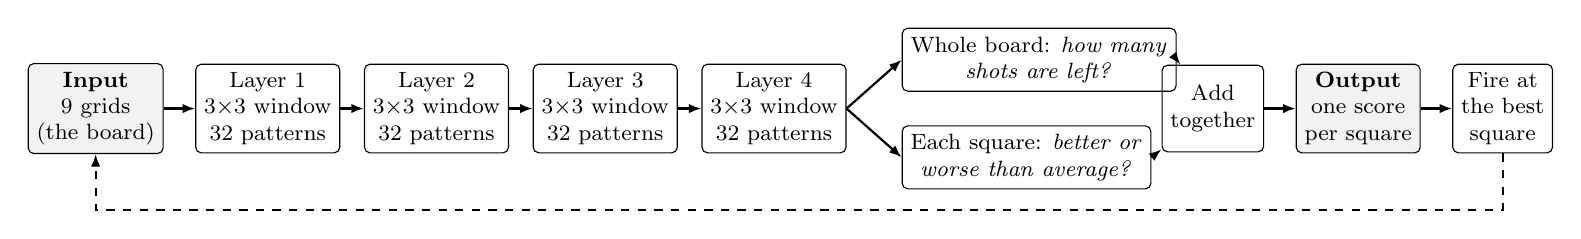
\begin{tikzpicture}[
  box/.style={draw, rounded corners=2pt, align=center, minimum height=1.1cm,
              inner sep=3pt, font=\footnotesize},
  arr/.style={-{Latex[length=1.6mm]}, thick}]
\node[box, fill=gray!10] (in) {\textbf{Input}\\9 grids\\(the board)};
\node[box, right=0.4cm of in] (l1) {Layer 1\\3$\times$3 window\\32 patterns};
\node[box, right=0.3cm of l1] (l2) {Layer 2\\3$\times$3 window\\32 patterns};
\node[box, right=0.3cm of l2] (l3) {Layer 3\\3$\times$3 window\\32 patterns};
\node[box, right=0.3cm of l3] (l4) {Layer 4\\3$\times$3 window\\32 patterns};
\node[box, right=0.7cm of l4, yshift=0.62cm, minimum height=0.8cm] (v)
  {Whole board: \emph{how many}\\\emph{shots are left?}};
\node[box, right=0.7cm of l4, yshift=-0.62cm, minimum height=0.8cm] (a)
  {Each square: \emph{better or}\\\emph{worse than average?}};
\node[box, right=0.6cm of l4, xshift=3.4cm] (q) {Add\\together};
\node[box, fill=gray!10, right=0.4cm of q] (out) {\textbf{Output}\\one score\\per square};
\node[box, right=0.4cm of out] (fire) {Fire at\\the best\\square};
\draw[arr] (in) -- (l1); \draw[arr] (l1) -- (l2); \draw[arr] (l2) -- (l3);
\draw[arr] (l3) -- (l4); \draw[arr] (l4.east) -- (v.west); \draw[arr] (l4.east) -- (a.west);
\draw[arr] (v.east) -- (q); \draw[arr] (a.east) -- (q);
\draw[arr] (q) -- (out); \draw[arr] (out) -- (fire);
\draw[arr, dashed] (fire.south) -- ++(0,-0.72) -| (in.south);
\end{tikzpicture}

\caption{The current network, used on both boards. Each layer widens the view by one square on each side; after each shot (dashed line) the new board goes back in.}
\label{fig:net}\end{figure*}

\section{Current Network, Layer by Layer}
Fig.~\ref{fig:net} shows the network. Each part has one job.
\begin{itemize}
\item \textbf{Input: 9 grids.} The board as it stands, one fact per grid: hits,
misses, sunk ships, the board's edge, and how many ships of each length are
still afloat.
\item \textbf{Layer 1.} Looks at each square and its 3$\times$3 neighbourhood
with 32 filters, small pattern detectors such as ``a hit beside me'' or ``a
miss beside me''. Each filter outputs a map of where its pattern appears, so the
layer passes 32 maps on.
\item \textbf{Layers 2--4.} Each combines the 32 maps from the layer before into
32 larger patterns, and widens the view by one square on each side: 5$\times$5,
7$\times$7, then 9$\times$9. Larger views can capture, for example, two hits in
a line, or a gap too short for any remaining ship. After layer 4, every square
sees far enough to tell whether a 5-square ship can pass through it. The
patterns are learned, not programmed.
\item \textbf{Whole-board estimate.} Summarises all squares into one number:
how many shots the game still needs.
\item \textbf{Per-square estimate.} Turns each square's 32 values into one
number: how much better or worse that square is than average.
\item \textbf{Output.} The two are added into one score per square. Squares
already fired at are blocked, and the agent fires at the best square. After
each shot the new board goes back in.
\end{itemize}

\section{Proposal: 2$\times$2 Windows on 4$\times$4}
\textbf{Why.} On 4$\times$4 the longest ship has 3 squares, so a 5$\times$5
view is enough. The current 9$\times$9 view mostly looks beyond the board's
edge, which wastes effort.

\textbf{What changes.} Only the four layers. Each looks through a 2$\times$2
window instead of 3$\times$3; the input, the 32 filters per layer and the
output stay the same. A 2$\times$2 window has no centre square, so it can only
look to one side~\cite{evenkernel}. The layers therefore take turns: one looks
right and down, the next left and up. Four such layers see a centred 5$\times$5
area, exactly what the small board needs. The window slides one square at a
time, so neighbouring windows overlap and every square keeps its own score.

\section{Next Actions}
\begin{enumerate}
\item \textbf{Build.} Add the 2$\times$2 window, with alternating directions, as
an option; existing trained agents stay unchanged. Test that the view is
centred.
\item \textbf{Train.} Train four versions on 4$\times$4, five times each:
\emph{A}, the current network; \emph{B}, two 3$\times$3 layers, which also
see 5$\times$5; \emph{C}, the 2$\times$2 proposal; and \emph{D}, 2$\times$2
blocks that do not overlap. B separates the effect of the window's shape from
the size of the view, and D checks whether overlap matters.
\item \textbf{Evaluate.} Each trained agent plays every possible 4$\times$4
board, and we compare the average number of shots to win.
\item \textbf{Report.} The current agent is already near the best possible
play, so the likely outcome is a smaller network that plays as well. The
10$\times$10 agent keeps 3$\times$3 windows, since 2$\times$2 would need twice
as many layers there.
\end{enumerate}

\section*{Acknowledgment}
We thank Akhilesh Kasturi for suggesting this experiment. Claude (Anthropic)
helped draft this proposal.

\begin{thebibliography}{1}
\bibitem{evenkernel} S. Wu, G. Wang, P. Tang, F. Chen, and L. Shi,
``Convolution with even-sized kernels and symmetric padding,'' in \emph{Proc.
NeurIPS}, 2019.
\end{thebibliography}

\end{document}
